\section{Examplary Content}
\label{chap:spring}
In order to advance the research and standardization of a flexible and universal source routing mechanism, the Internet Engineering Task Force (IETF) has formed a working group (WG) in 2013. This WG, called \emph{Source Packet Routing in Networking (SPRING)}, is chartered to identify source routing use cases as well as defining the requirements and mechanisms for implementing, deploying and administrating source routing enabled networks \cite{springcharter}. The working group yet developed a new source routing mechanism called \emph{segment routing} \cite{spring-sr-10}, which is discussed in section \ref{sec:spring-sr}. It further introduced two implementational approaches \cite{spring-ipv6,spring-mpls}, which will be discussed in section \ref{sec:spring-mpls} and \ref{sec:spring-ipv6}. The working group is currently preparing their final document revisions for a technical review and adoption to IETF standards track \cite{springstatus}.

\subsection{Segment Routing}
\label{sec:spring-sr}
Segment routing is a new source routing mechanism developed by the IETF SPRING working group. It is based on so-called \emph{segments} \cite{spring-sr-10}. The SPRING architecture \cite{spring-sr-10} defines that a segment represents \emph{"an instruction a node executes on the incoming packet (e.g.: forward packet according to shortest path to destination, or, forward packet through a specific interface, or, deliver the packet to a given application/service instance)"}. A segment and its associated \emph{Segment Identifier (SID)} is advertised within the segment routing domain with the help of the Interior Gateway Protocol (IGP) in use. Therefore the SPRING working group has defined extensions for the IGP protocols OSPF \cite{spring-ospf}, OSPFv3 \cite{spring-ospfv3} and IS-IS \cite{spring-isis}. With the help of these extensions, those protocols are able to carry the necessary segment routing signaling information. Segment routing introduces three major types of segments \cite{salsano2015pmsr,spring-sr-10}:
\begin{itemize}
	\item IGP-Prefix Segments
	\item IGP-Node Segments
	\item IGP-Adjacency Segments
\end{itemize}
Each of these segment types are discussed in the following sections. The term \emph{ingress node} identifies the node at which a packet enters the segment routing domain, whereas \emph{egress node} identifies the node at which a packet exits the segment routing domain.

\subsubsection{IGP-Node Segment}
\label{sec:nodal-segment}
An IGP-node segment has global scope and thus is identified by a globally unique SID. Each node is assigned a SID and advertises its nodal segment via the IGP protocol \cite{packet-pushers-sr-intro}. Global scope in this context means that all nodes within a segment routing domain add an entry in their Forwarding Information Base for the instruction associated with that segment \cite{cisco-whitepaper}. The node identified by the node-SID is always reached by the shortest path, which is determined by the IGP algorithm \cite{spring-sr-10}. That means an ingress node can impose a source route to a packet by specifying another node to be traversed by prepending the correspondent node-SID to that packet.
\newline
\newline
Figure \ref{fig:node-segment} shows an exemplary scenario: Node R advertised its node-SID $70$ to all other nodes within the domain. Node S can instruct incoming packets to traverse node R by prepending the node-SID $70$ to it. Hence the packet will be either forwarded via the path \{S,A,B,R\} or \{S,C,D,R\}, depending on which of both paths have been investigated as the shortest path. Intermediate nodes do not change the prepended SID, thus symbolically swapping it from $70$ to $70$, except for the last node. The last node on the path towards R is directly connected to R and thereby can remove the SID as this information is not needed anymore \cite{packet-pushers-sr-intro}.

\begin{figure}%[h]
	\centering
	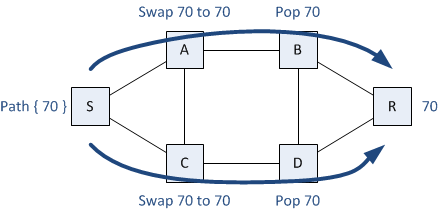
\includegraphics[width=0.95\linewidth]{figures/node-segment-2.png}
	\caption{Node Segments \cite{packet-pushers-sr-intro}}
	\label{fig:node-segment}
\end{figure}